\documentclass{article}
\usepackage{times}
\usepackage{amsmath}
\usepackage{mathptmx}
\usepackage{textcomp}
\usepackage{graphicx}
\usepackage{color}
\usepackage{xspace}
\usepackage[caption=false]{subfig}
\usepackage{multirow}
\usepackage[compact]{titlesec}
\usepackage{float}
\usepackage{epstopdf}
\usepackage{balance}



\setlength{\textwidth}{6.5in}
\setlength{\textheight}{9.50in}
\setlength{\oddsidemargin}{-.19in}
\voffset=-1.0in

\title{CS 690LG Project: Distributed SAT Solving}
\author{Prateek Sharma}


\begin{document}
\maketitle
\section{Introduction}

The Boolean satisfiability problem (SAT) has many real-world
applications and solving it is extremely important. Although it is NP
complete, even large SAT instances are now solvable, mainly due to
advances in heuristics and a better understanding of the structure of
SAT problems. SAT has a growing list of applications. Traditionally,
it has been used for hardware and software verification (like model
checking) and general theorem proving (prover9/mace4). More recently,
SAT solvers are being used in areas ranging from computational biology
to bitcoin mining.


Since SAT is NP-complete, the only way to solve it is a worst-case
exponential search. Let an SAT instance be denoted as $(V,C)$, where V
is the set of variables $\{x_1,x_2,\ldots x_n \}$, and C is the set of
clauses. One of the original SAT solving approaches was
DPLL~\cite{knuth}, which is a basic backtracking search in this
exponential search space. The DPLL approach has proven to be
remarkably useful, and even after more than 50 years, some industrial
SAT solvers still use some variant of it, although Conflict Driven
Clause Learning (CDCL) is increasingly popular.


The large computation time required to solve SAT instances has been
conveniently provided by Moore's law and Dennard Scaling, which
resulted in faster clockspeed. However, recent hardware architectures
have strongly veered towards more parallelism in the CPUs (via
multiple CPU cores), and larger clusters of commodity hardware. This
means that computationally intensive tasks now have to be performed in
a distributed manner. The ubiquity and low-cost of cloud computing
services such as Amazon's EC2, where users can launch a cluster of
1000s of machines in a minute at a very low cost, also means that the
cloud is a cost-effective platform for computationally intensive tasks
like SAT solving.


In order to take advantage of clusters of computers, SAT solvers have
to be distributed. This is not a new challenge, and has received
significant attention. There are two main techniques that parallel SAT
solvers use:

\begin{enumerate}
\item \textbf{Portfolio Approach: } Each solver thread operates on the
  entire input problem, but with different heuristics. Threads
  therefore ``compete'' with one another to solve the same problem
  instance. The portfolio approach at first seems wasteful and naive,
  because it attempts to explore a large search space by running the
  multiple searches in parallel and hoping that one of them gets
  lucky.

\item \textbf{Divide and Conquer: } Either the problem instance or the
  solution space is divided among the threads, and each thread thus
  operates on a different search space. Division of the search space
  is non trivial, and balancing the workloads of multiple threads is a
  nuisance in this approach because some threads can be stuck with a
  ``hard'' portion of the search space.
\end{enumerate}


\subsection{Project Scope \& Contributions}

In this project report, I will study and extend
ManySAT~\cite{hamadi2008manysat}, a parallel SAT solver. ManySAT is a
DPLL porfolio based solver which utilizes multiple threads. I will
show the performance characteristics of ManySAT on SAT benchmarks, and
compare it to a recent world-champion solver,
plingeling~\cite{plingeling}.


ManySAT is restricted to working on a single machine, and is not
capable of distributed operation. I will also develop a distributed
version of ManySAT, called dManySAT, which can utilize a cluster of
machines. I will show the design and implementation of my distributed
version, along with preliminary performance results.


\section{Background: ManySAT}

ManySAT is a DPLL (backtracking) based solver which spwans mulitple
threads, all attacking the same search space. Each thread, however,
has different heuristics, which enable the search to proceed in
different order. Below is a description of the various components of the solver:

\textbf{Input: } ManySAT takes a SAT instance in the DIMACS format as
the input, along with other solver configuration parameters. The input
instance is fed to SatElite for pre-processing.


\textbf{Parallelism: } Parallelism is provided by using multiple
\emph{threads} to solve the input instance. The number of threads can
be user specified, but defaults to the number of cores available on
the machine. Threads are implemented by using the OpenMP API. Each
thread is given the entire input problem instance to solve, and the
program terminates if any thread has finished solving the instance
(either a satisfying assignment or proving that it is Unsatisfiable).


\textbf{Portfolio: } ManySAT originally employed a portfolio of
heuristics for the different threads. For example, different threads
have different restart and decision variable choosing heuristics
(VSIDS). However, the recent ManySAT implementation (version 2.0),
also provides a \emph{deterministic mode} of operation, in which all
the threads use the same heuristics, except for the decision
variables. That is, the threads use different decision variables at
each step in the search.


\textbf{Restart: } If a thread is ``too deep'' into the search space,
then the solver restarts its search (from the very
beginning). Restarts are a crucial component of all modern SAT
solvers, and avoid the solvers from getting stuck in some useless part
of the search space. ManySAT has implemented many restart heuristics,
and uses the Luby~\cite{luby} policy by default.

\textbf{Clause learning: } During the course of a search, ManySAT uses
a CDCL-like scheme for learning clauses. These learnt clauses are used
when the thread is restarted.

\textbf{Clause sharing: } Knowledge sharing is the crucial component
of parallel solvers, and allows threads to learn from each
other. Clause sharing in ManySAT is performed just before a thread
restarts. The set of learnt clauses is kept in a global (shared by all
threads) structure. Before a restart, a thread exports the clauses
learnt in the prior run and imports clauses from other threads,
applies these learnt clauses to its local input instance, and then
restarts the search, armed with new and potentially useful
knowledge. 

The flip-side of sharing knowledge is that the number of sharing the
clauses can be detrimental to performance because of the overheads
involved with sharing and storing all the shared clauses. Pruning the
shared clauses is essential to reduce the overhead due to sharing and
memory requirements. ManySAT addresses this by providing
user-controllable configuration parameters to limit the number of
clauses imported by threads from other threads. If the limit is
crossed, then no more clauses are shared. This limit is applied
pairwise among threads, so a thread may not accept any new clauses
from thread-A, but can do so from thread-B, if the number of shared
clauses from thread-B is still under the limit.


Another mechanism provided by ManySAT to control clause sharing is to
restrict the size of the clauses shared. The user can specify (via the
\texttt{limitEx} option, the maximum size of the clauses considered
for sharing. The default maximum size of shared clauses is 10. The
relation between performance and clause sharing will be evaluated in
the evaluation section. Clause sharing is an important design
component and will be explored in depth later when discussing the
distributed ManySAT implementation.


\section{Design of dManySAT}

This section describes the distributed solver developed as part of
this course project. The solver is based on ManySAT, and gives it the
ability to operate in a distributed manner (hence the name). Since
ManySAT is portfolio based, it is easier to parallelize. The threads
operate independently for the most part, only communicating before
restarts when they exchange clauses. The rest of this section
describes the clause sharing.


\textbf{Interface: } The command-line based user-interface of ManySAT
remains. dManySAT is launched on all the nodes of the cluster with the
same problem instance. 

\subsection{Communication}

ManySAT threads do not communicate much with each other, which is good
news for the distributed implementation.

\textbf{Thread Start:} Thread starts across different machines are not
synchronized. Each solver starts independently, there is no barrier. 


\textbf{Finish: } When a thread has found the answer, it terminates
the solver on the local machine. The result is copied to the other
machines, and their solvers are terminated via \texttt{ssh}.

\subsection{Clause Sharing}

Clause sharing among different threads on the same machine is the same
as ManySAT. Unit clauses and clauses of longer length are shared among
threads before restarts via a shared in-memory data structure. In
ManySAT, this is a 2-d array  of pointers to vectors of clauses. For each
pair of threads $(s,t)$, there is a vector of clauses that $s$ has
learnt from $t$. The clause sharing among local threads has not been
modified. The shared data structure is protected by an OpenMP barrier. 


Clause sharing between machines is the interesting part, and received
a significant portion of the effort in the design and implementation
phase of this project. 

The basic design principle for clause sharing is fairly simple. On
each machine, one thread from the thread-pool is ``stolen'' from the
solver, and instead acts as the communication thread. This
communication thread sends and receives clauses across the
network. When the threads on a machine restart, they perform their
local clause sharing as usual. After the local clause sharing is over,
they then perform clause sharing with other machines (via the
communication thread) as follows.


Exporting clauses to other machines is performed by broadcasting the
clause to all the machines. On each machine, the communication thread
receives and stores these broadcast clauses. 

Once learnt clauses have been exported, a thread then \emph{imports}
clauses from other threads. Here too, clauses from local threads are
imported first. Then, the clauses are imported from the communication
thread. Remember that the communication thread receives broadcasts
from all the threads from all the machines. During the import, the
local threads pull the clauses from the communication thread. 


The communication thread maintains a buffer of received clauses which
is cleared when local threads have already merged these clauses into
their instances. In ManySAT, all clauses are shared between all
threads (as long as they are under the sharing quotas). However, this
threatens to overwhelm threads with too many learnt clauses, because
the communication thread has a large number of clauses from all the
machines in its buffers. 

This ``too many shared clauses'' problem is mitigated by using two techniques:

\begin{enumerate}
\item The input buffer in the communication thread is of a fixed size and maintained in a FIFO manner.
\item Instead of sharing the clauses with all the local threads,
  dManySAT only shares the remotely-learnt clauses with $k$ of $n$
  threads. The first $k$ solver threads to ask the communication
  thread for clauses are given all the clauses, and then the input
  buffer is cleared. This has two advantages. First, not all threads
  are burdened with a large number of learnt clauses. Second, the
  buffer is more frequently cleared because we dont have to wait for
  all the $n$ threads to ask for the shared clauses. In the current
  implementation, $k=n/2$. 
\end{enumerate}




\section{Implementation}

dManySAT is implemented by modifying ManySAT, and requires about 500
lines of C++ code. 

Communication among machines is done over the network by the
communication threads. Many communication platforms were contemplated,
tried, and abandoned: MPI, zeroMQ. MPI is the defacto HPC
communication interface, but sadly proved to be too restrictive when
combined with ManySAT's existing clause sharing design. The primary
goal of the implementation was to minimize the amount of changes to
ManySAT. The solution finally adopted was to use simple BSD TCP
sockets to send and receive clauses. The communication thread
maintains a list of open sockets to the other machines (the peers),
and broadcasts clauses by sending them to all the peers.


Since clauses are sent over the network, care it taken to serialize
them and convert from host to network byte order, etc. ManySAT clauses
are simply a vector of literals. ManySAT has its own vector
implementation (not \texttt{std::vector}), which is quite amenable to
network communication and did not require a serialization library like
protobufs. A manysat vector is simply an array with the size as the
first element. Thus, to send a clause, the clause vector is just sent
over the wire. Unit clauses are represented by literals, which are
again plain integers. ManySAT uses a single integer to encode both the
variable and the polarity. Unit literals are converted to unit clauses
(by prefixing the size=1) and then sent.


The communication thread constantly listens on its receive socket, and
places all clauses on the input buffer. There are separate sockets for
receiving and broadcasting. The input buffer is filled in by the
communication thread, and drained by the other solver threads, and is
protected by an OpenMP mutex. 


Exporting a clause implies a message-send, which is simply a socket
send after converting to a safe binary format. Currently, dManySAT
broadcasts clauses eagerly without any buffering, which adds to the
networking overhead. A simple optimization would be to buffer exported
clauses and send bigger messages.



general theorem proving, comp bio, verification. efficiency gains 100k var, millions of clauses. algo improvements and better understanding of the structure. 



considerably much more advanced and sophisticated
performance enhancements have been algorithmic (VSIDS, conflict clause learning,..) 
watched literal lists 

Dist solvers: gridsat~\cite{chrabakh2003gridsat}, pasat, paMIRA~\cite{schubert2005pamira}, 

Multithreaded sat solving~\cite{lewis2007multithreaded}

In many fields from verification to AI, mapped to CNF. All variables
undefined, then constraint propagation (DPLL) backtracking,

conflict clauses can be exchanged

gridsat used MPI 

ingredients: restarts, branching, conflict analysis, clause db cleaning

all threads working on same proof Solver(sigma) 

clauses are sent as soon as they are learnt . NOT 

UNSAT things too? 

Seven challenges~\cite{hamadi2013seven}. knowledge sharing

partitioning techniques: ~\cite{hyvarinen2010partitioning}

SAT solvers have become powerful tools to tackle problems ranging from
verification, combinatorial challenges, bitcoin mining, etc.

portfolio: let threads compete 

d and c: divide search space or decompose the formula. Workload balancing is hard 

larger portfolio needs better heuristics and more diverse 

FUTURE: combine manysat and plingeling?

shared knowledge on restarts 

restart policies prevent search from getting stuck 

manysat: pairwise size limits. plingeling only shares unit clauses! plingeling won sat-11

manysat2.0: first decision variables are different, that is all! size 10 and below 

plingeling ~\cite{biere2010lingeling}

dimacs : vars clause ; then the clause themselves one per line 






\section{Evaluation}

To evaluate the performance of ManySAT, I used the Sat-Competition
2014~\cite{sc14} benchmarks. In particular, since SAT solvers are
usually used for specific applications, I used the ``application''
benchmarks from the benchmark suite.


A major problem with SAT is that many instances require too much
time. When I ran the full application benchmark suite to sanity-check
ManySAT, some problems ran for over two days(!). For the rest of the
experiments, I have used a timeout value of 1000 seconds, and problems
taking longer than that are terminated. From the full benchmark suite,
only \textbf{26} problems finished within 100 seconds, and all the
experiments were performed on each of these 26 problems.


The hardware platform used for all the experiments was a Dell
PowerEdge R210 server with 16GB memory and 8 core Xeon E3-1240 V2
CPU. This CPU has hyperthreading enabled (thus 8 effective CPUs). Some
of the experiments were also performed on a newer, 6th generation
Intel CPU (Core i5-6500) to test whether ManySAT can take advantages
of the newer architecture and new instruction set. The ManySAT program
was compiled by GCC with the \texttt{-O3} optimization flag.


\textbf{plingeling:} In addition to evaluating my modifications to
ManySAT, I also compared with plingeling, the parallel version of
lingeling, which is the 2011 SAT contest winner and a very competitive
industrial SAT solver. Plingeling is CDCL based, and only shares unit
clauses.



\subsection{Experiment Platform}
Experiment setup

\begin{figure}[h]
  \centering
  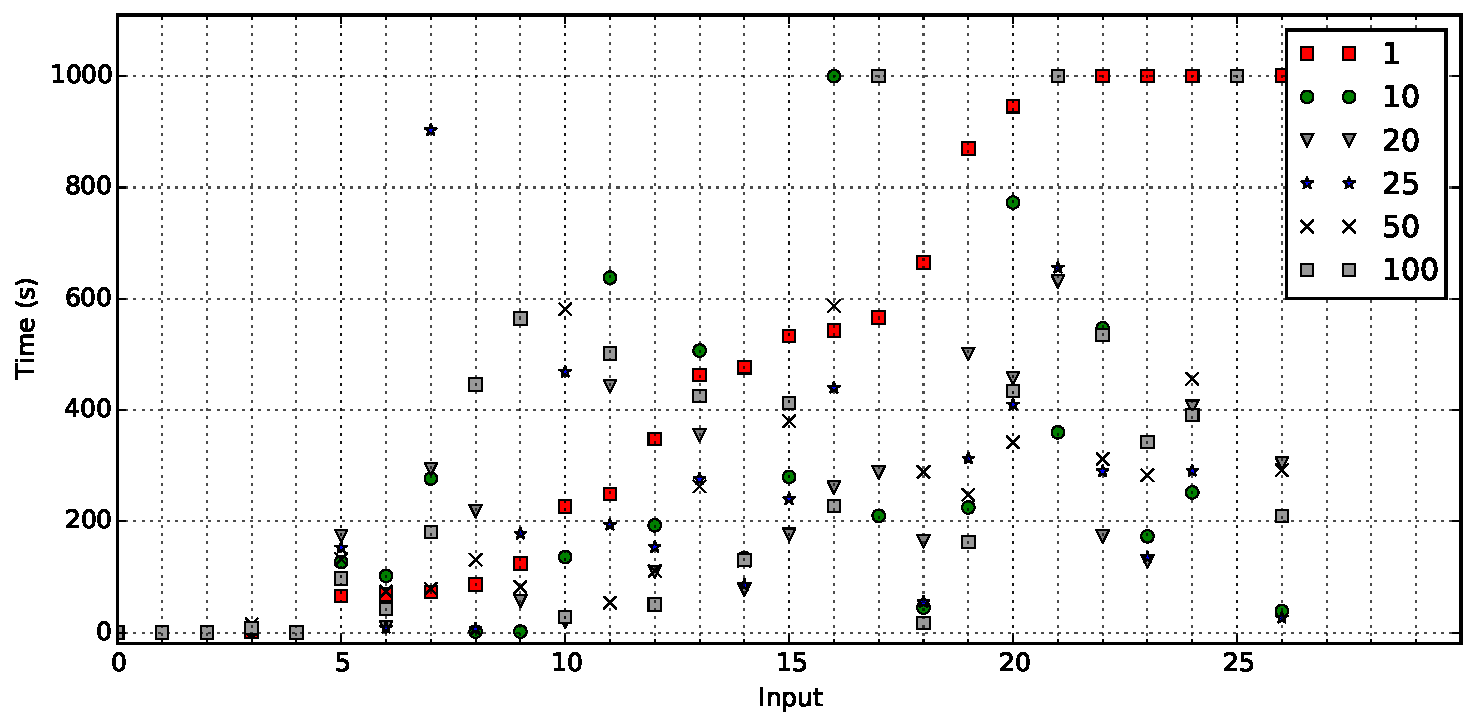
\includegraphics[width=0.8\textwidth]{../figs/scatter_all.pdf}
  \caption{Scatter-plot of running times.}
  \label{fig:scatter-1}
\end{figure}


\begin{figure}[h]
  \centering
  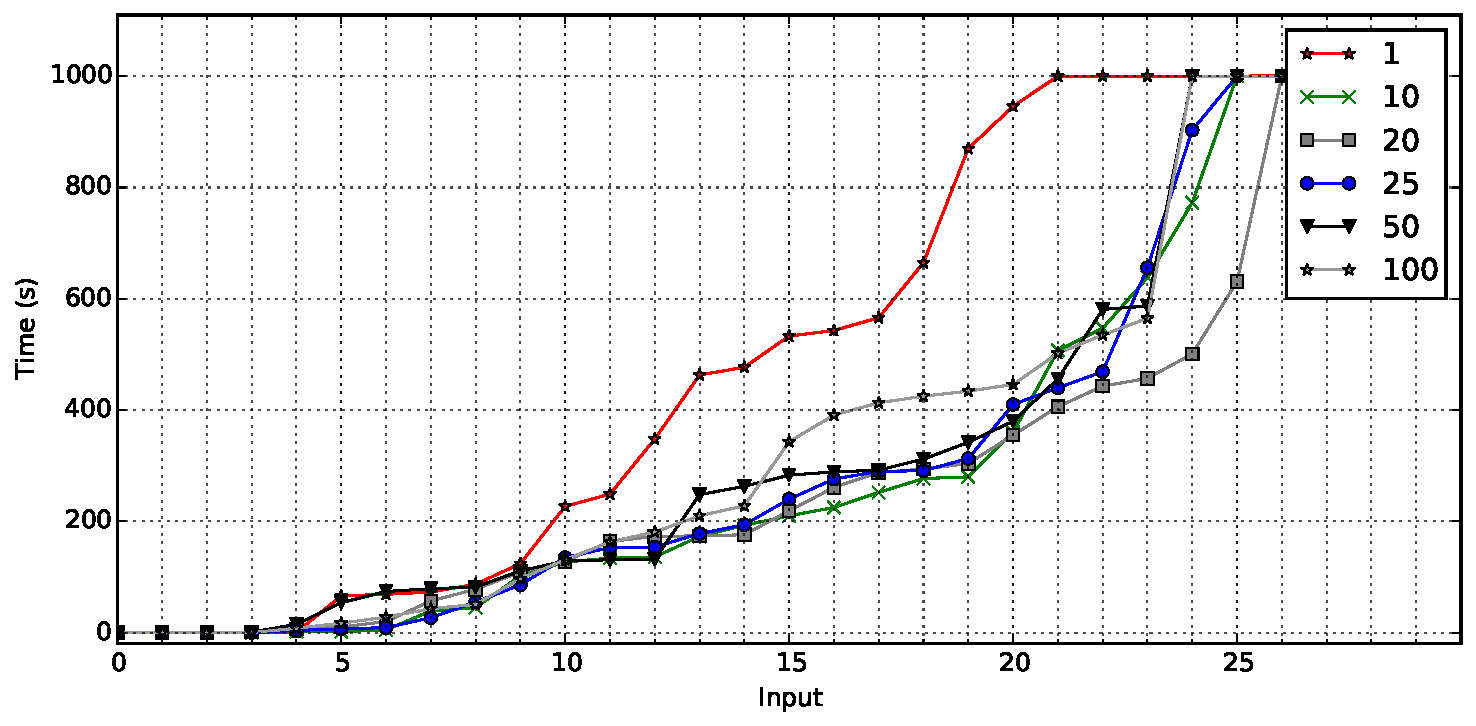
\includegraphics[width=0.8\textwidth]{../figs/scatter_cdf.pdf}
  \caption{CDF of running times of ManySAT with different clause sharing limits}
  \label{fig:scatter-2}
\end{figure}


\begin{figure}[h]
  \centering
  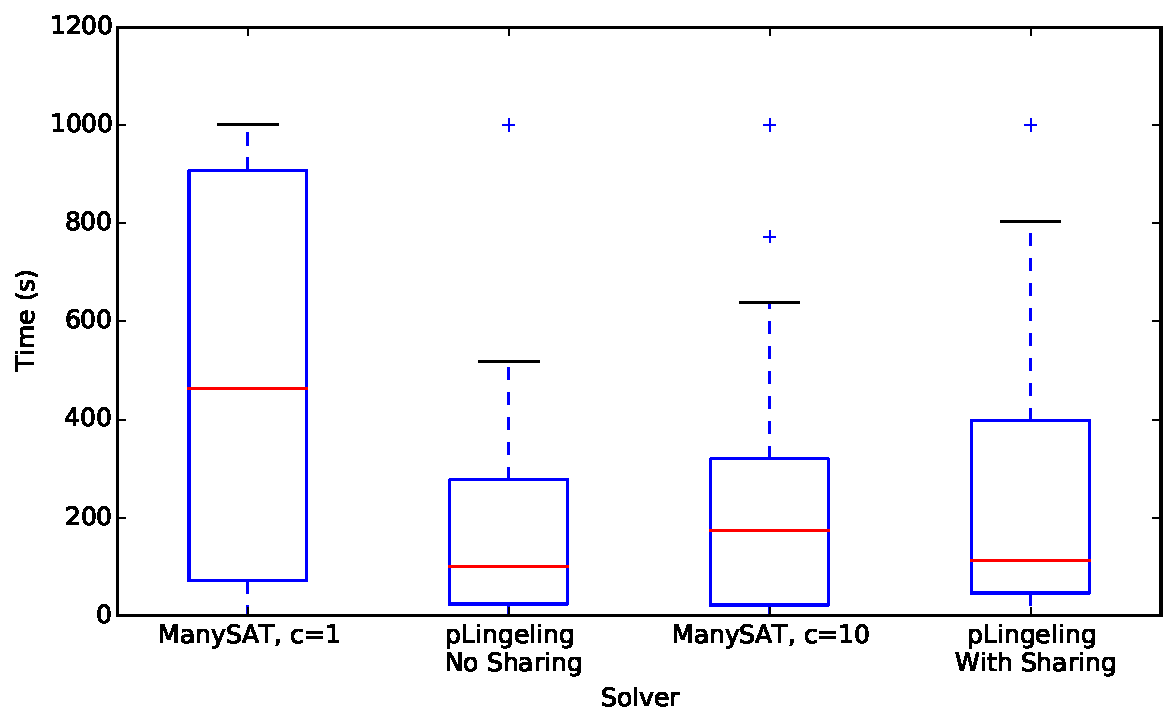
\includegraphics[width=0.8\textwidth]{../figs/cmp_box.pdf}
  \caption{Effect of clause sharing on ManySAT and plingeling.}
  \label{fig:cmp-1}
\end{figure}

\begin{figure}[h]
  \centering
    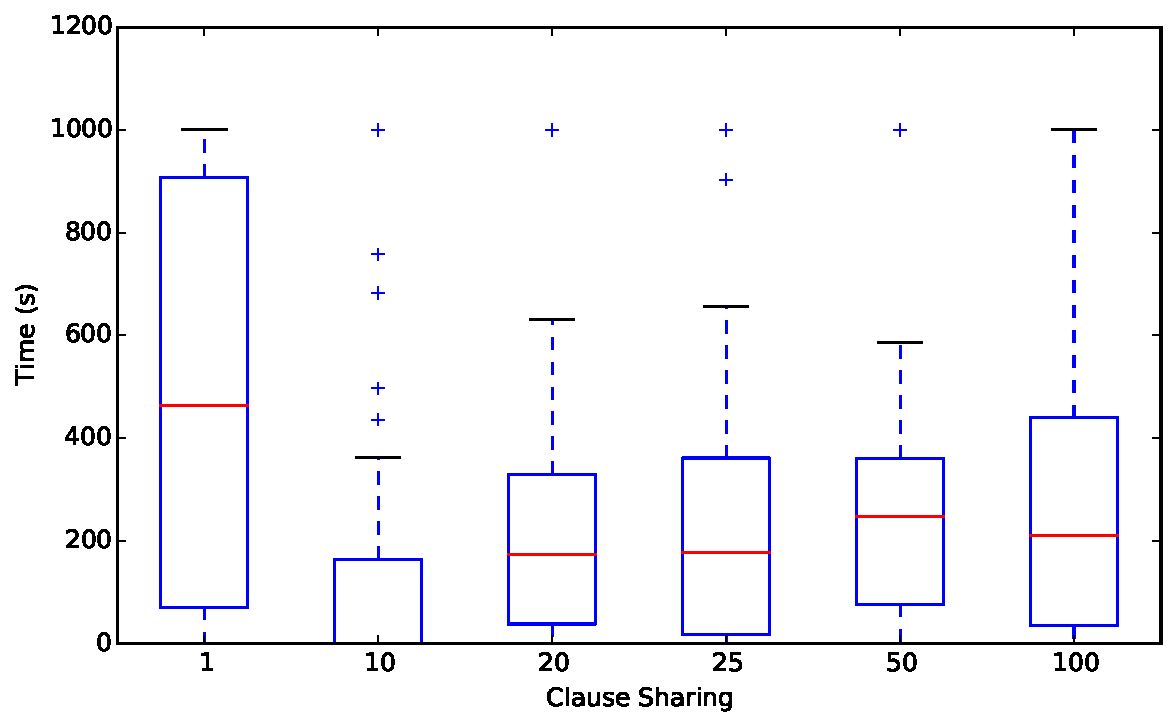
\includegraphics[width=0.8\textwidth]{../figs/boxplot_all.pdf}
  \caption{Summary of running times. Default clause length of 10 yields best results. Sharing only unit clauses hurts performance significantly.}
  \label{fig:boxplot-1}
\end{figure}



\begin{figure}[h]
  \centering
  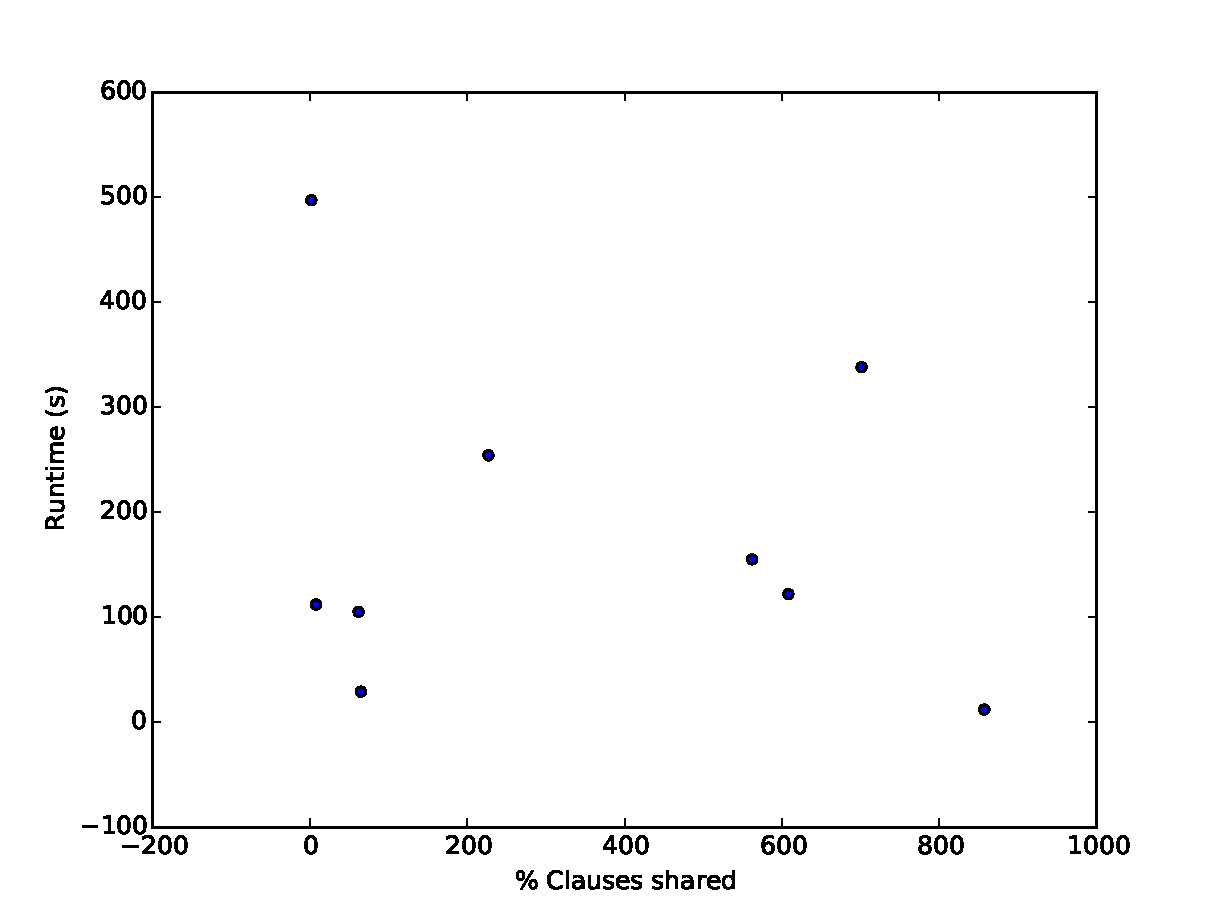
\includegraphics[width=0.8\textwidth]{../figs/gss-18-s100.pdf}
  \caption{Percentage of clauses shared vs running time for gss-18-s100 input}
  \label{fig:gss}
\end{figure}

average about 11k variables and 60k clauses
max 53k variables , 161k clauses

\bibliographystyle{plain}
\bibliography{parsat}


\end{document}